% Misión 2: inspección de un pilar. Portada y vuelo paso a paso.
% El pilar está en NED norte 8, este 6.5; la hélice tiene radio 3 m y sube de 1 a 4 m en 3 vueltas.
% Empieza en el punto del círculo más cercano al despegue: a 219° (desde el norte, hacia el este).

\begin{frame}{Misión 2: inspección de un pilar}
  \begin{columns}[c]
    \column{0.56\textwidth}
    \begin{tikzpicture}
      \node[inner sep=0] (im) {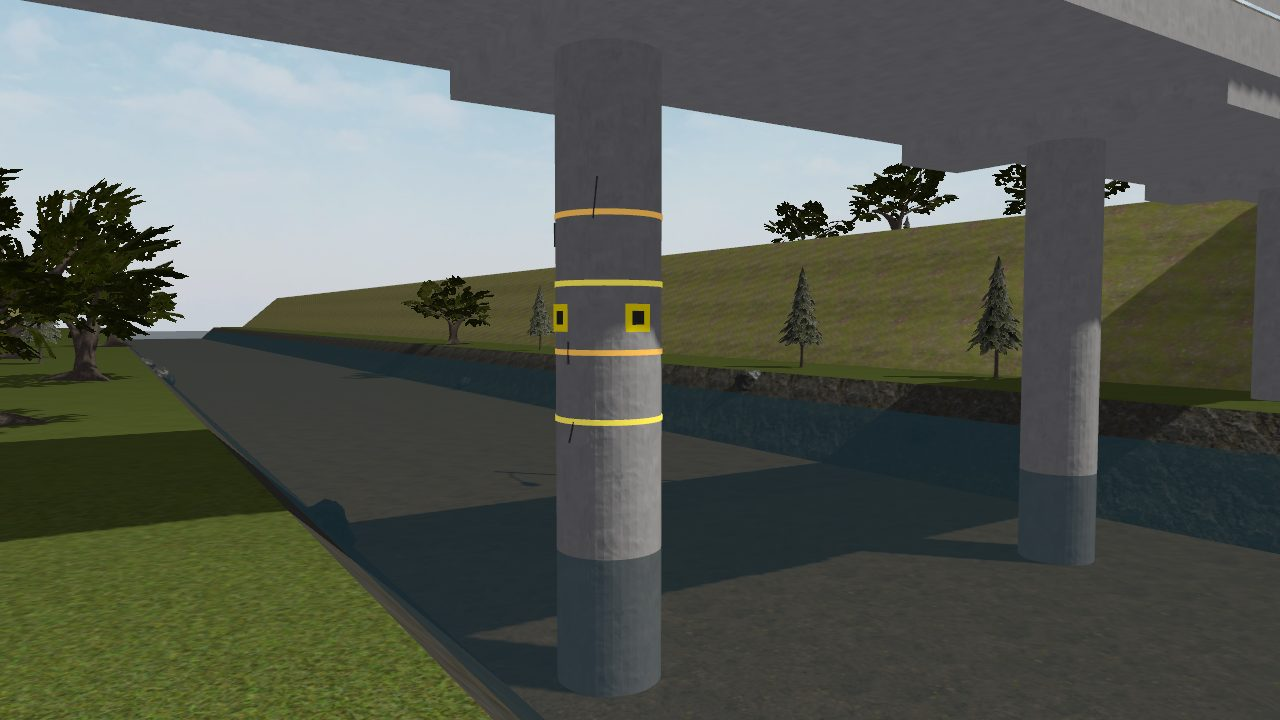
\includegraphics[width=\linewidth]{puente_rio_pilar}};
      \node[anchor=north west,fill=azul,text=white,font=\bfseries\scriptsize,rounded corners=2pt]
        at ([xshift=4pt,yshift=-4pt]im.north west) {MISIÓN 2 · NIVEL 1 \nivel{1}};
    \end{tikzpicture}\\[0.3em]
    \small\textbf{Escenario}: una constructora necesita fotos de un pilar del puente \textbf{desde todos los
    ángulos y alturas}. El dron sube en hélice alrededor, con la nariz (la cámara) siempre al pilar.
    \column{0.41\textwidth}
    \ficha{x500_volando}{x500}{puente\_rio}{inspeccion\_pilar}{\cmd{orbit\_mission} y \cmd{figure\_eight}}%
      {posición + velocidad (feedforward) y yaw al centro}{radio $3 \pm 0.3$ m, yaw \textless 10°, 3 vueltas, 4 m}
  \end{columns}
\end{frame}

\begin{frame}{La hélice, paso a paso}
  \begin{columns}[c]
    \column{0.31\textwidth}\centering
    {\scriptsize\textbf{desde arriba}}\\
    \begin{tikzpicture}[scale=0.36]
      \draw[gray!20,step=1] (-1.5,-1.5) grid (10.5,12);
      \draw[-{Stealth},verde,thick] (0,-1.5) -- (0,12.3) node[above,font=\tiny] {N};
      \draw[-{Stealth},rojo,thick] (-1.5,0) -- (10.8,0) node[right,font=\tiny] {E};
      \node[draw,circle,fill=azulclaro,inner sep=0.5pt,font=\tiny] at (0,0) {H};
      \draw[azul!50,thick] (6.5,8) circle (3);
      \fill[gray!70] (6.5,8) circle (0.8);
      \draw[azul,dashed,thick,-{Stealth},visible on=<2>] (0.4,0.6) -- (4.5,5.4);
      \draw[azul,dashed,thick,-{Stealth},visible on=<6>] (4.5,5.4) -- (0.4,0.6);
      % ángulo theta desde el norte; el dron mira al pilar: yaw = theta + 180
      \only<1,6-7>{\node at (0,0) {\dronarriba{1cm}};}
      \only<2-3>{\node[rotate=-39] at ({6.5+3*sin(219)},{8+3*cos(219)}) {\dronarriba{1cm}};}
      \only<4>{\node[rotate=-159] at ({6.5+3*sin(339)},{8+3*cos(339)}) {\dronarriba{1cm}};}
      \only<5>{\node[rotate=-279] at ({6.5+3*sin(99)},{8+3*cos(99)}) {\dronarriba{1cm}};}
    \end{tikzpicture}
    \column{0.2\textwidth}\centering
    {\scriptsize\textbf{de lado}}\\
    \begin{tikzpicture}[scale=0.62]
      \fill[green!35!black!40] (-1.6,-0.15) rectangle (1.6,0);
      \fill[gray!35] (-0.3,0) rectangle (0.3,5.2);
      \foreach \h/\c in {1/rojo,2/naranja,3/verde,4/azul} \fill[\c] (-0.3,\h-0.06) rectangle (0.3,\h+0.06);
      \foreach \h in {1,2,3,4} \node[font=\tiny,left] at (-1.6,\h) {\h\,m};
      \draw[azul!60,thick,domain=0:1080,samples=150,smooth,variable=\t,visible on=<3->]
        plot ({1.2*sin(\t)}, {1+\t/360});
      \only<1>{\node[anchor=south] at (1.2,0) {\dronlado{0.75cm}};}
      \only<2-3>{\node at (1.2,1) {\dronlado{0.75cm}};}
      \only<4>{\node at (1.2,2.5) {\dronlado{0.75cm}};}
      \only<5>{\node at (1.2,4) {\dronlado{0.75cm}};}
      \only<6>{\node at (1.2,1) {\dronlado{0.75cm}};}
      \only<7>{\node[anchor=south] at (1.2,0) {\dronlado{0.75cm}};}
    \end{tikzpicture}
    \column{0.47\textwidth}
    \estados{1/SUBIR,2/ACERCAR,3-5/HÉLICE,6/REGRESAR,7/LANDING}
    \vspace{0.3em}

    \only<1>{\begin{terminal}{inspeccion\_pilar}
inspeccion\_pilar: 3.0 vueltas de radio 3.0 m,\\
\ \ de 1.0 a 4.0 m, 57 s\\
OFFBOARD activo, subiendo a 1.0 m
    \end{terminal}\small Sube sobre el despegue a la altura de la primera banda.}%
    \only<2>{\begin{terminal}{inspeccion\_pilar}
Arriba, acercándome al pilar
    \end{terminal}\small Va al punto del círculo \textbf{más cercano} al despegue: así no rodea el pilar para
      llegar.}%
    \only<3>{\begin{terminal}{inspeccion\_pilar}
En el punto de inicio, empezando la hélice
    \end{terminal}\small Vuelta 1. La nariz \textbf{apunta al pilar} desde el principio.}%
    \only<4>{\small Vuelta 2: \textbf{gira y sube al mismo tiempo}. El nodo manda posición, velocidad y
      \cmd{yawspeed} en cada ciclo (feedforward), así no se queda atrás.}%
    \only<5>{\small Vuelta 3, llegando a 4 m. Mientras vuela, el nodo mide el radio y el yaw
      \textbf{reales} contra la tolerancia.}%
    \only<6>{\begin{terminal}{inspeccion\_pilar}
Hélice completa, regresando sobre el despegue
    \end{terminal}}%
    \only<7>{\begin{terminal}{inspeccion\_pilar}
vueltas: 2.99 de 3.00 OK\\
altura máxima: 3.99 m de 4.00 m OK\\
error máximo de radio: 0.11 m (límite 0.30) OK\\
error máximo de yaw: 6.1° (límite 10°) OK\\
Misión cumplida
    \end{terminal}}%
  \end{columns}
\end{frame}
